% Options for packages loaded elsewhere
\PassOptionsToPackage{unicode}{hyperref}
\PassOptionsToPackage{hyphens}{url}
%
\documentclass[
  ignorenonframetext,
]{beamer}
\usepackage{pgfpages}
\setbeamertemplate{caption}[numbered]
\setbeamertemplate{caption label separator}{: }
\setbeamercolor{caption name}{fg=normal text.fg}
\beamertemplatenavigationsymbolsempty
% Prevent slide breaks in the middle of a paragraph
\widowpenalties 1 10000
\raggedbottom
\setbeamertemplate{part page}{
  \centering
  \begin{beamercolorbox}[sep=16pt,center]{part title}
    \usebeamerfont{part title}\insertpart\par
  \end{beamercolorbox}
}
\setbeamertemplate{section page}{
  \centering
  \begin{beamercolorbox}[sep=12pt,center]{part title}
    \usebeamerfont{section title}\insertsection\par
  \end{beamercolorbox}
}
\setbeamertemplate{subsection page}{
  \centering
  \begin{beamercolorbox}[sep=8pt,center]{part title}
    \usebeamerfont{subsection title}\insertsubsection\par
  \end{beamercolorbox}
}
\AtBeginPart{
  \frame{\partpage}
}
\AtBeginSection{
  \ifbibliography
  \else
    \frame{\sectionpage}
  \fi
}
\AtBeginSubsection{
  \frame{\subsectionpage}
}

\usepackage{amsmath,amssymb}
\usepackage{iftex}
\ifPDFTeX
  \usepackage[T1]{fontenc}
  \usepackage[utf8]{inputenc}
  \usepackage{textcomp} % provide euro and other symbols
\else % if luatex or xetex
  \usepackage{unicode-math}
  \defaultfontfeatures{Scale=MatchLowercase}
  \defaultfontfeatures[\rmfamily]{Ligatures=TeX,Scale=1}
\fi
\usepackage{lmodern}
\ifPDFTeX\else  
    % xetex/luatex font selection
\fi
% Use upquote if available, for straight quotes in verbatim environments
\IfFileExists{upquote.sty}{\usepackage{upquote}}{}
\IfFileExists{microtype.sty}{% use microtype if available
  \usepackage[]{microtype}
  \UseMicrotypeSet[protrusion]{basicmath} % disable protrusion for tt fonts
}{}
\makeatletter
\@ifundefined{KOMAClassName}{% if non-KOMA class
  \IfFileExists{parskip.sty}{%
    \usepackage{parskip}
  }{% else
    \setlength{\parindent}{0pt}
    \setlength{\parskip}{6pt plus 2pt minus 1pt}}
}{% if KOMA class
  \KOMAoptions{parskip=half}}
\makeatother
\usepackage{xcolor}
\newif\ifbibliography
\setlength{\emergencystretch}{3em} % prevent overfull lines
\setcounter{secnumdepth}{-\maxdimen} % remove section numbering


\providecommand{\tightlist}{%
  \setlength{\itemsep}{0pt}\setlength{\parskip}{0pt}}\usepackage{longtable,booktabs,array}
\usepackage{calc} % for calculating minipage widths
\usepackage{caption}
% Make caption package work with longtable
\makeatletter
\def\fnum@table{\tablename~\thetable}
\makeatother
\usepackage{graphicx}
\makeatletter
\def\maxwidth{\ifdim\Gin@nat@width>\linewidth\linewidth\else\Gin@nat@width\fi}
\def\maxheight{\ifdim\Gin@nat@height>\textheight\textheight\else\Gin@nat@height\fi}
\makeatother
% Scale images if necessary, so that they will not overflow the page
% margins by default, and it is still possible to overwrite the defaults
% using explicit options in \includegraphics[width, height, ...]{}
\setkeys{Gin}{width=\maxwidth,height=\maxheight,keepaspectratio}
% Set default figure placement to htbp
\makeatletter
\def\fps@figure{htbp}
\makeatother

\makeatletter
\@ifpackageloaded{caption}{}{\usepackage{caption}}
\AtBeginDocument{%
\ifdefined\contentsname
  \renewcommand*\contentsname{Table of contents}
\else
  \newcommand\contentsname{Table of contents}
\fi
\ifdefined\listfigurename
  \renewcommand*\listfigurename{List of Figures}
\else
  \newcommand\listfigurename{List of Figures}
\fi
\ifdefined\listtablename
  \renewcommand*\listtablename{List of Tables}
\else
  \newcommand\listtablename{List of Tables}
\fi
\ifdefined\figurename
  \renewcommand*\figurename{Figure}
\else
  \newcommand\figurename{Figure}
\fi
\ifdefined\tablename
  \renewcommand*\tablename{Table}
\else
  \newcommand\tablename{Table}
\fi
}
\@ifpackageloaded{float}{}{\usepackage{float}}
\floatstyle{ruled}
\@ifundefined{c@chapter}{\newfloat{codelisting}{h}{lop}}{\newfloat{codelisting}{h}{lop}[chapter]}
\floatname{codelisting}{Listing}
\newcommand*\listoflistings{\listof{codelisting}{List of Listings}}
\makeatother
\makeatletter
\makeatother
\makeatletter
\@ifpackageloaded{caption}{}{\usepackage{caption}}
\@ifpackageloaded{subcaption}{}{\usepackage{subcaption}}
\makeatother
\ifLuaTeX
  \usepackage{selnolig}  % disable illegal ligatures
\fi
\usepackage{bookmark}

\IfFileExists{xurl.sty}{\usepackage{xurl}}{} % add URL line breaks if available
\urlstyle{same} % disable monospaced font for URLs
\hypersetup{
  pdftitle={Welcome!},
  hidelinks,
  pdfcreator={LaTeX via pandoc}}

\title{Welcome!}
\subtitle{PM 566: Introduction to Health Data Science}
\author{}
\date{}

\begin{document}
\frame{\titlepage}

\begin{frame}{Instructor}
\phantomsection\label{instructor}
\begin{itemize}
\tightlist
\item
  Kim Siegmund
\end{itemize}
\end{frame}

\begin{frame}{Blackboard + Website}
\phantomsection\label{blackboard-website}
https://github.com/USCbiostats/PM566\\
Official class website Syllabus, reading materials, slides, labs and
assignments

https://blackboard.usc.edu/\\
Announcements + Grading
\end{frame}

\begin{frame}{USC Software Development Help Page}
\phantomsection\label{usc-software-development-help-page}
https://uscbiostats.github.io/software-dev-site/

collection of knowledge about

\begin{itemize}
\tightlist
\item
  computing
\item
  standards
\item
  research practices
\end{itemize}
\end{frame}

\begin{frame}{What is data science?}
\phantomsection\label{what-is-data-science}
\begin{itemize}
\tightlist
\item
  Data science is an exciting discipline that allows you to turn raw
  data into understanding, insight, and knowledge.
\end{itemize}

--

.center{[} 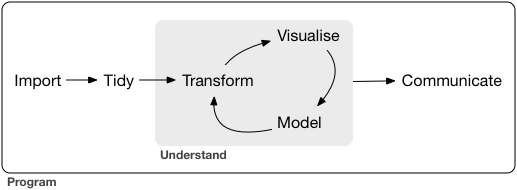
\includegraphics{img/data-science.png}{]}
\end{frame}

\begin{frame}
Source:
https://berkeleysciencereview.com/2013/07/how-to-become-a-data-scientist-before-you-graduate/
Original by Drew Conway.
\end{frame}

\begin{frame}{Data science can be really cool}
\phantomsection\label{data-science-can-be-really-cool}
Source: https://xkcd.com/208/
\end{frame}

\begin{frame}{With great power comes great responsibility}
\phantomsection\label{with-great-power-comes-great-responsibility}
Fuente: https://xkcd.com/605/
\end{frame}

\begin{frame}
(Also see
\href{https://www.amstat.org/asa/News/New-Report-Highlights-Growing-Demand-for-Data-Science-Analytics-Talent.aspx}{here},
and \href{https://www.ibm.com/downloads/cas/3RL3VXGA}{here}, and
\href{https://www.forbes.com/sites/gilpress/2021/06/27/salaries-and-job-opportunities-for-data-scientists-continue-to-rise/}{here},
and \href{https://www.glassdoor.com/research/job-market-report/}{here} )
\end{frame}

\begin{frame}{What is this course?}
\phantomsection\label{what-is-this-course}
This course is a introduction to the world of data science with a focus
on application in the health sciences.

--

The course will teach language agnostic skills that are easily
transferable, with examples done in R.

--

You can use any language/tool you prefer. But we can only guarantee help
if you are using R and RStudio.
\end{frame}

\begin{frame}{What is R?}
\phantomsection\label{what-is-r}
\begin{quote}
R is a language and environment for statistical computing and graphics.
---https://r-project.org
\end{quote}

Created by statisticians for statisticians.

Over 16,000 packages added to CRAN
\end{frame}

\begin{frame}
\begin{block}{What is RStudio?}
\phantomsection\label{what-is-rstudio}
\begin{quote}
RStudio is an integrated development environment (IDE) for R. ---
https://www.rstudio.com/products/rstudio/
\end{quote}
\end{block}
\end{frame}

\begin{frame}
\end{frame}

\begin{frame}
\begin{block}{R in the terminal}
\phantomsection\label{r-in-the-terminal}
\end{block}
\end{frame}

\begin{frame}
\begin{block}{R + RStudio}
\phantomsection\label{r-rstudio}
\end{block}
\end{frame}

\begin{frame}{Break time}
\phantomsection\label{break-time}
Following break we will run lab 01
\end{frame}

\begin{frame}{First Lab}
\phantomsection\label{first-lab}
The lab exercises can be found at:

Website -\textgreater{} Schedule -\textgreater{}

\includegraphics[width=1.25em,height=1em]{week1_files/figure-beamer/fa-icon-324241782d9e44e9978a25bf05b1d0cd.pdf}
-\textgreater{} Lab Exercise

https://uscbiostats.github.io/PM566/labs/lab-01/01-lab.html

Related Github Issue

https://github.com/USCbiostats/PM566/issues/54
\end{frame}



\end{document}
